%&pdflatex
\documentclass[12pt,a4paper]{article}
\usepackage[left=1in,right=1in, bottom=1in]{geometry}
\usepackage[utf8]{inputenc}
\usepackage[english]{babel}			%other options: frenchb,german
\usepackage[pdftex]{graphicx}
\usepackage{moreverb}
\usepackage[hidelinks]{hyperref}
\usepackage{titling}
\usepackage{caption}
\usepackage{listings}

% move title to top of page
\setlength{\droptitle}{-10em}

% remove additional space between tables and their captions
\captionsetup[table]{skip=0pt}
\graphicspath{{figures/}}

% title setup
\title{Robotics Challenge 2015}
\date{May 28, 2015}
\author{
	Fabienne \textsc{Gürtler}\\
	IN.2022 Robotics, BSc Course, 2nd Sem.\\
	University of Fribourg \\
	\href{mailto:fabienne.guertler@unifr.ch}{fabienne.guertler@unifr.ch}
}

% setup page
\sloppy
\pagenumbering{roman}
\pagestyle{plain}
\pagenumbering{arabic}
\pagestyle{headings}

\begin{document}
%################### Report Start #####################################
\maketitle

\section*{Introduction}
This project requires multiple robots to work together to solve a problem. They communicate through events which they send each other.

\section{Problem statement}
%Description of the challenge and the environment (e-puck robots, ASEBA suite, and lab).
There are 3 e-pucks in an arena. In this arena there are 2 blue doors and 4 red switches. To open a door a switch must be pressed, meaning to pass through a door two e-pucks have to work together. One finds either the door or the switch and waits in front of it while the other searches the missing component. Once both the door and the switch have been found the door opens and the e-puck can pass. Another requirement for the challenge is that all e-pucks must have the same code, except for calibration values. Before I begin presenting one of the many possible solution strategies I'll present the e-puck and the arena in detail.

\paragraph{E-puck}
The Ecole Polytechnique Fédérale de Lausanne started the e-puck project with the main goal to develop a miniature mobile robot for educational purposes. The design of the e-puck (Figure \ref{fig:epuck}) is based on desktop size and flexibility. By default it comes with sound sensors, a 3D accelerometer, 8 proximity sensors and a camera. It is possible to extend the e-puck with more hardware like a Color LED Communication Turret, ground sensors, magnetic wheels and more. For this project we used e-pucks with ground sensors. The e-pucks communicate via Bluetooth. An e-puck is a event-based robot, it can both receive and emit events.

\begin{figure}[h!]
\begin{center}
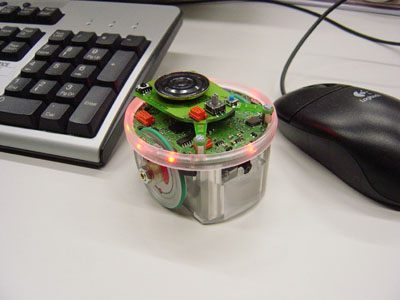
\includegraphics[width = 5cm]{images/epuck-look.jpg}
\caption{E-puck}
\label{fig:epuck}
\end{center}
\end{figure} 


\begin{figure}[h!]
\begin{center}
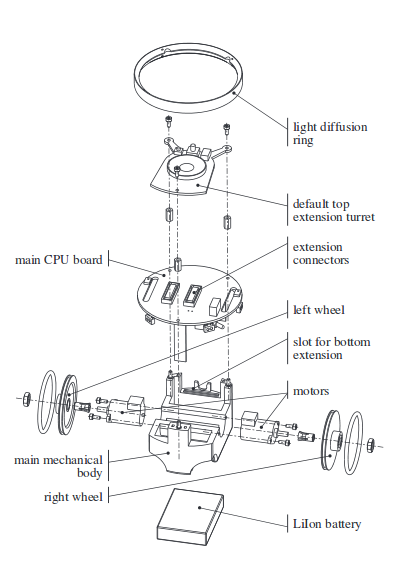
\includegraphics[scale=0.5]{images/epuck-concept.png}
\caption{Mechanical structure}
\label{fig:epuck structure}
\end{center}
\end{figure} 

\noindent The structure (Figure \ref{fig:epuck structure}) is based on one single part to keep the desing simple and elegant. This basic part has a diameter of 7 cm and supports the motor, the circuit and the battery. The e-puck uses a miniature stepper motor with gear reduction and the wheels have a diameter of 4,1 cm. 

\paragraph{Arena}
The arena is a 80cm x 160cm zone divided into two subspaces of roughly the same area. Both the floor and the walls are white. In the area there are the following randomly placed objects:
\begin{itemize}
	\item 2 blue doors, equipped with black stripes on the floor
	\item 4 red switches, two per subspace
	\item three epucks
\end{itemize}

\paragraph{Software}
For the completion of the project we used the help of two programs, Aseba Studio and Aseba Playground.\\
\textit{Aseba Playground} simulates the arena, enabling us to test the robots behaviour virtually before trying to program the real robots. We did not use it very much because the color recognition works very differently in the simulation than in reality.\\
\textit{Aseba Studio} is the programming environment used to program the e-pucks. It let's you load code onto one or more e-puck and execute it.


\section{Solution Strategy} \label{sec:solStrategy}
%Description of the approach chosen to solve the challenge.
\subsection{Basic Idea}
The principle of our solution is to manage the e-puck's behaviour with the three variables \textit{redFound, blueFound} and \textit{color}. Figure \ref{fig:behaviour code} illustrates this idea.

\begin{figure}[h!]
\begin{center}
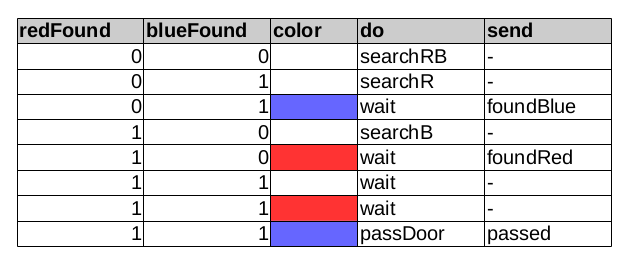
\includegraphics[scale=0.5]{images/behaviourCode.png}
\caption{Coding for e-puck behaviour}
\label{fig:behaviour code}
\end{center}
\end{figure}

\noindent While neither color has been found the e-puck searches for both. If the e-puck knows that one color was found but does not see it himself he searches for the missing color. If he is the one who found the color he waits in front of the object until released. It is easiest to use an example to illustrate:\\

\noindent \textit{redFound = True; blueFound = False; color = no color:} The e-puck knows that the color red was found so he stops searching it and instead only looks for the color blue. 
Once he found red he sets \textit{blueFound} to True and is in the constellation \textit{redFound = True; blueFound = True; color = blue}. This means that both colors were found and he is standing in front of the door, which he can now begin to pass. As soon as that is done he emits the command \textit{passed} which releases the variables, thus making the e-puck start searching again. 
The \textit{do} column represents the states a e-puck can have and the send column are the events he sends to the other e-pucks.\\ \\
This is the basic version of the project and it uses only two colors. It can already be used for three e-pucks as we defined a state where both colors were found but the e-puck sees no color. In this first version the third e-puck simply waits for the other to finish their routine. We later expanded the third e-puck's behaviour. Ideas for expansions with a third color are discussed later in this article. With this strategy it is relatively easy to expand the code for more colors. 

\subsection{Final strategy}
Our first logic worked fairly well so we kept most of it. In fact, we only added some additional cases to better handle a third e-puck. The final logic is shown in Figure \ref{fig:logic table}

\begin{figure}[h!]
\begin{center}
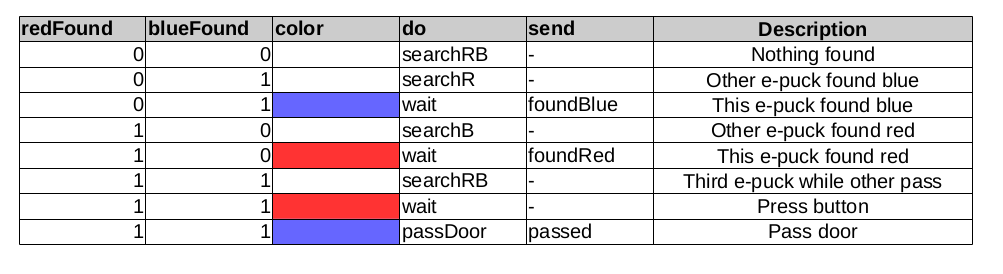
\includegraphics[scale=0.5]{images/LogicTable.png}
\caption{Logic table}
\label{fig:logic table}
\end{center}
\end{figure}

\noindent We changed the behaviour for the third e-puck for when the other two have found both colors and started passing the door. Now the third e-puck no longer just waits until they are done, but now already starts looking for both colors again. If he finds a color he waits until they completed their procedure and then emits the event that he found a color. This speeds up the whole process because the third e-puck may already begin to search while the other are in the passing respectively the pressing the button state thus increasing the speed with which the objects are found. The process shown here is infinite so we also introduced a point system to define a end for the game.
For successfully passing a door the e-puck gets 2 points and for pressing a switch he gets 1 point. We decided to give points to both participants but to give more points to the one passing the door because it is harder than pressing a switch. The e-puck that first reaches 7 points is the winner and emits the victory event upon which all e-pucks start "dancing" with the winner blinking all his leds.

\subsection{State machine}
From the logic table in Figure \ref{fig:logic table} we came up with our state machine (Figure \ref{fig:State Machine}).

\begin{figure}[h!]
\begin{center}
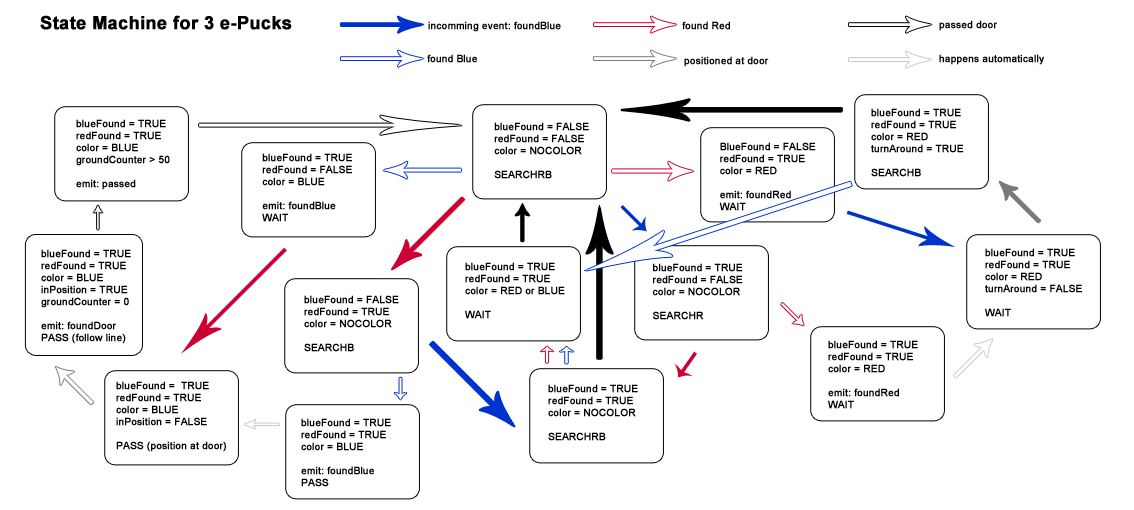
\includegraphics[width = \linewidth]{images/StateMachine.png}
\caption{State Machine}
\label{fig:State Machine}
\end{center}
\end{figure}

\paragraph{States}
Our state machine has the following states:
\begin{itemize}
	\item SEARCHRB:	nothing found yet $\rightarrow$ search both colors
	\item SEARCHR:	Someone else found blue $\rightarrow$ search red
	\item SEARCHB:	Analogue searchR but with red
	\item PASS:		Both colors found. In front of blue $\rightarrow$ pass the door
	\item WAIT:		Either found object or press button $\rightarrow$ wait
	\item VICTORY:	E-puck got at least 7 points $\rightarrow$ dance
\end{itemize}

\paragraph{Events}
\begin{itemize}
	\item foundRed:	Camera recognized red and approached it $\rightarrow$ set redFound = True
	\item foundBlue:	analogue foundRed
	\item passed:	Passed the door $\rightarrow$ reset controlling variables to False  
	\item victory:	Emitter won $\rightarrow$ dance  
\end{itemize}

\begin{figure}[h!]
\begin{center}
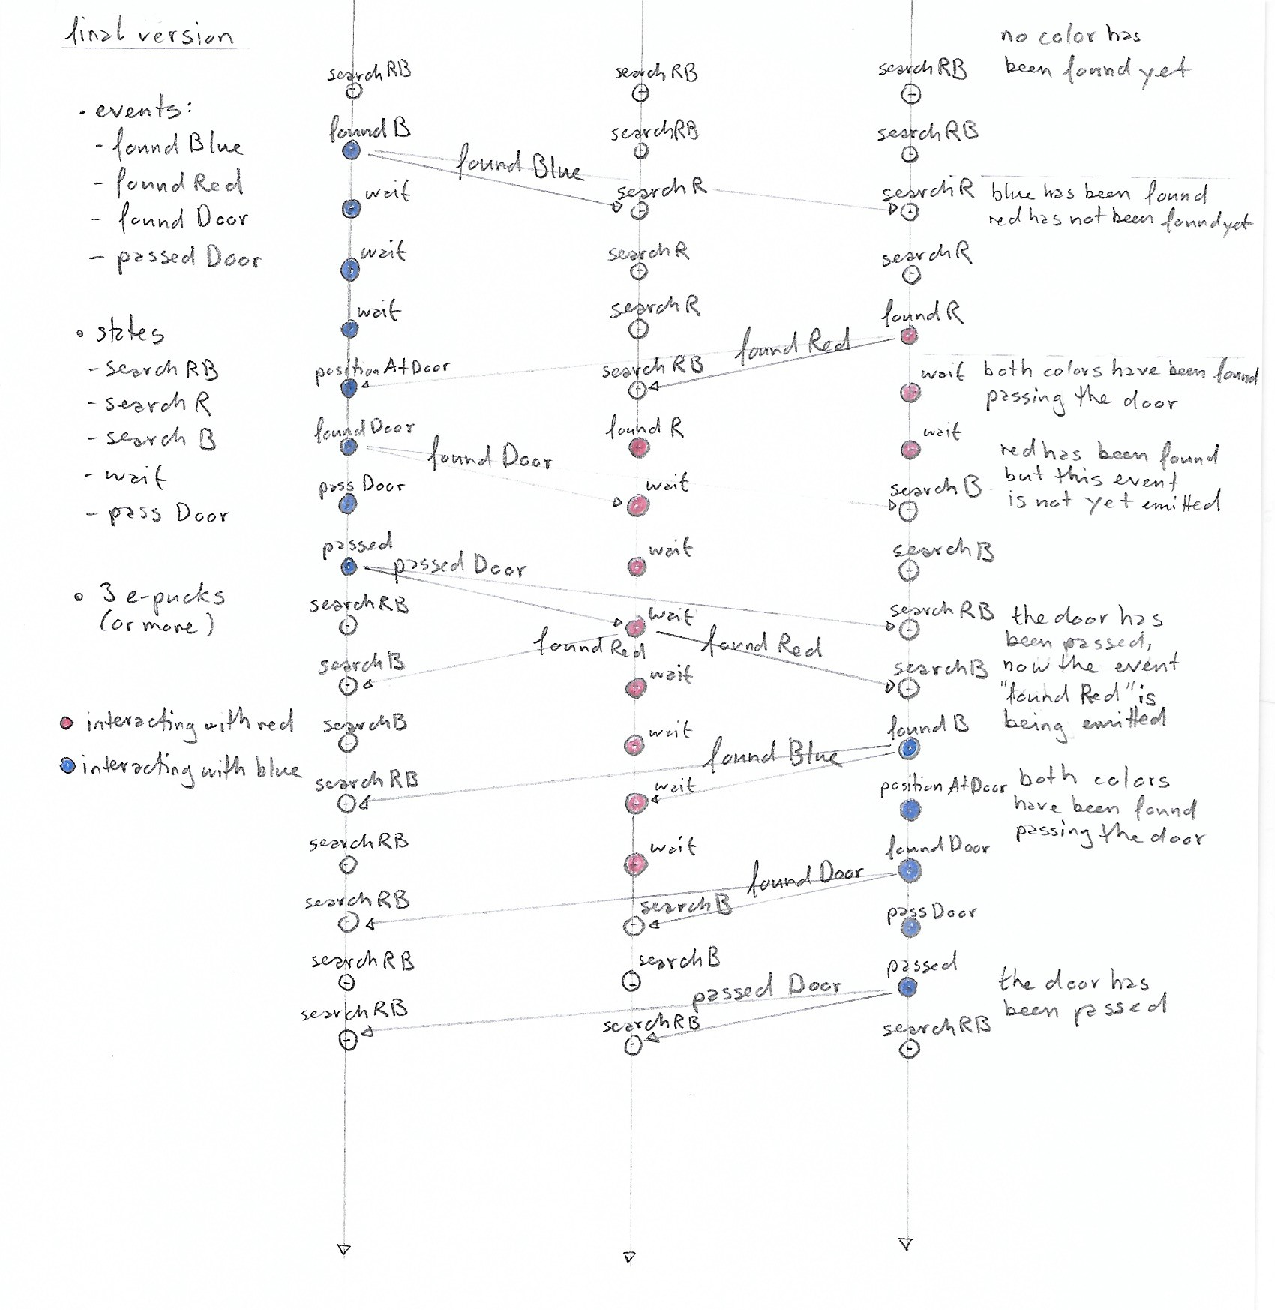
\includegraphics[scale=0.5]{images/linediagramfinal.pdf}
\caption{Event diagram}
\label{fig:Line diagram}
\end{center}
\end{figure}

\section{Implementation}
The implementation is pretty straight forward from the state machine. In fact we had bigger problems to implement the behaviours themselves than to implement the main logic connecting them. Once we managed to get all subroutines to work we could see that our logic worked as intended.
\paragraph{Control variables}
The main controllers of our project are 
\begin{itemize}
	\item redFound: True if red was found by either himself or another e-puck. False otherwise
	\item blueFound: like redFound but for blue
	\item color: stores color he found. Used to check whether he is the finder of the object
\end{itemize}
Taking a look at the implementation, many commonalities to the logic table can be noted.
\begin{lstlisting}
onevent ir_sensors
	[...]
	# both colors were found -> pass door
	elseif redFound == TRUE and blueFound == TRUE and
	   	color == BLUE then
	   	leds[0] = 1
		leds[2] = 0
		leds[4] = 0
		leds[6] = 0
		state = PASS
\end{lstlisting}

\paragraph{Secondary variables}
In addition to these main controller variables we introduced some helper variables. They are not an essential part of the logic but were needed to implement the behaviours. 
\begin{itemize}
	\item camColor: Color camera sees at this moment
	\item gameOver: True if one e-puck reached 7 points, false otherwise
	\item turnAround: helper variable used after press button to make e-puck turn. 
	\item inPosition: True if e-puck found black stripe and is ready to pass the door
\end{itemize}

\noindent We had to differentiate between camColor and color because for example while passing the door the camera no longer sees the color blue once the door was taken away. To ensure it still stays in the pass state defined in the logic table color needs to stay blue. So most of the time camColor and color are one and the same but not always. It also helps with fluctuation when searching. \\
Once the door was passed all main controller variables are reset meaning all e-pucks start searching red and blue. Of course this means that the e-puck that pressed the button would immediately find red again since it is standing in front of it. We found that a bit boring so we used the turnAround variable to make the e-puck turn around once the door is open. To implement this we made the e-puck at the door emit an event foundDoor once he found the black strip (inPosition = True) and is ready to follow the line.
\begin{lstlisting}
if not(v[0] < -50 and v[0] > -75) or 
   not(v[2] < -50 and v[2] > -75) then
	[...]
	emit foundDoor
\end{lstlisting}

\noindent If the receiver is in front of the switch he sets turnAround to true, otherwise he doesn't react.

\begin{lstlisting}
onevent foundDoor
	if color == RED then
		[...]
		turnAround = TRUE
	end
\end{lstlisting}
All the variable turnAround does is force the e-puck to search for blue while it is true. So from the moment the e-puck at the door sends that he is on the line until he sends the passed event the e-puck at the door searches for blue making him turn away from the switch. Of course this implies that the switch doesn't need to keep being pressed for the door to stay open.  

\subsection{Code structure}
The main subroutines are searchRB, searchR, searchB, passDoor and wait. They represent the states. The code structure is shown in Figure \ref{fig:Subroutines}
\begin{figure}[h!]
\begin{center}
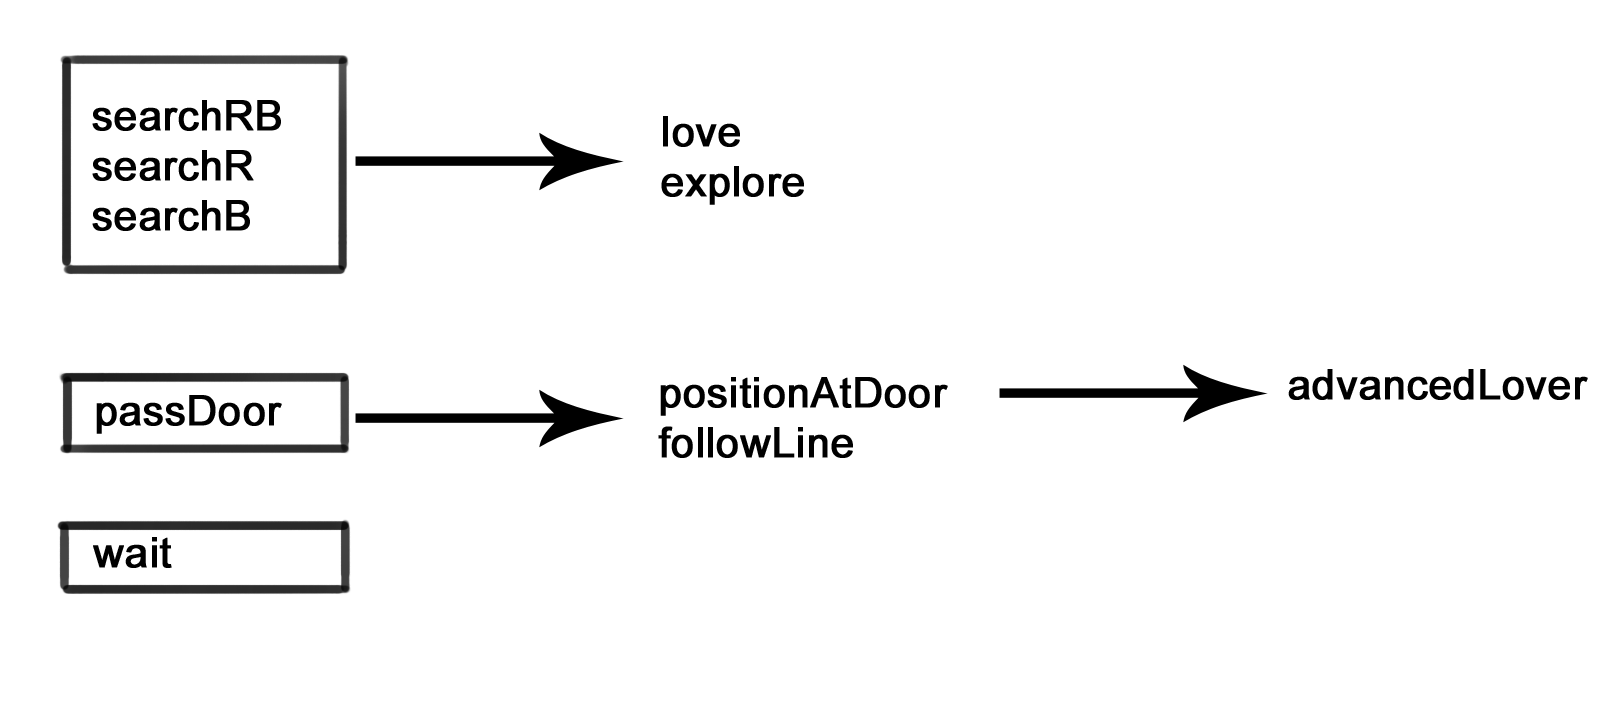
\includegraphics[scale=3]{images/SubroutinesOverview.png}
\caption{Subroutines}
\label{fig:Subroutines}	
\end{center}
\end{figure}
The only really new concepts are the positionAtDoor and the followLine subroutines, everything else is taken either from the sample solution of series 3 or is code form series 6. Which is why I will not discuss those in much detail. 

\subsection{Search functions}
For obvious reasons the search algorithms are essential for the project. The best logic or follow line implementation is useless when the e-puck does not find the objects. In other words how good or bad the color recognition works plays a big role in the success or failure of the whole project. This means every time we wanted to work with the e-pucks in the arena, we had to recalibrate the color recognition beforehand. To do so used the color recognition of an earlier series and adjusted the calibration values. The search functions are quite simple to implement and with a good calibration they worked reliably.
\begin{lstlisting}
sub searchRB
	if camColor == RED then
		callsub love

	elseif camColor == BLUE then
		callsub love
		
	else
		callsub explore
	end
\end{lstlisting}

\noindent The implementations for searchR and searchB work analogue. Once he spots the desired color he approaches it with the love behaviour, which makes him approach the object up to a certain distance. He then goes to the wait state and emits the corresponding found event if it has not been found already. 
\begin{lstlisting}
sub love
	[...] calculate proximity and delta-speed	
	# approach object, stop when in certain distance
	if proxTotal < P_THRESH_LOVE then	
	speed.right = SPEED_NORM - ds_left
	speed.left = SPEED_NORM - ds_right
	
	# only emit found when object wasn't found already
	else
		if camColor == BLUE and blueFound == FALSE then
			color = BLUE
			blueFound = TRUE
			emit foundBlue
		[...]
		end
		callsub wait
	end
\end{lstlisting}

\subsection{Pass Door}
The passDoor subroutine is called when the e-puck is waiting in front of the door and the switch has been found. Since the e-puck doesn't necessarily stand on the line it first calls a getInPosition subroutine which is tries to move him onto the black strip. Once it is in position it calls the followLine subroutine. \\\\
The idea for the getInPosition function was to let the e-puck drive along the wall with the advanced lover until he stands on the line but it does not quite work as we wanted. The problem is that because of the advanced lover it may get on the strip vertically. We could have let the e-puck make a 90 degree turn towards the door to fix this but unfortunately I did not think of this when we implemented it. This is probably the weakest part of our code and if we had more time I would definitely work on improving it. \\
The followLine subroutine works better than the positioning so if the e-puck stands in a good angle to the door it manages to pass the door. Like with the search algorithms a good calibration is very important to make a good line follower. We also used a short program to get the ground values and used that to find the range for black respectively white. Also the actual line following subroutine is only called once he is in position, meaning he has at least one wheel on the line. The line following itself is simple: if the ground sensor on the left (v[0]) leaves the stripe the e-puck turns right and if the sensor on the right leaves black it turns left. If both sensors leave the stripe it has passed the door. We used a variable groundCounter as a buffer because if both sensors are half on the stripe and half on the table it sometimes thinks both are on the table. Without the buffer it would then immediately send the passed event. Now every time both sensors are on white the groundCounter is incremented and once this counter reaches 50 it emits passed and starts searching again.
\begin{lstlisting}
sub followLine
	call ground.get_values(v)
	# 0 & 2 not on line
	if (v[0] < -55 and v[0] > -70) and 
	   (v[2] < -55 and v[2] > -70) then
		groundCounter++
	
	# 0 not on line
	elseif (v[0] < -55 and v[0] > -70) then
		speed.left = 200
		speed.right = 70
		groundCounter = 0

	# 2 not on line
	elseif [...]

	else # both on line
		speed.left = 200
		speed.right = 200
	end
		
	if groundCounter > 50 then
		[...]
		emit passed
		end
	end
\end{lstlisting}

\section{Validation}
%Description of how the solution turned out and what problems were encountered. Since this report is accompanied by a short video, it can be referenced to illustrate the result.
Our implementation more or less manages to solve the basic  problem. A demonstration can be seen in the video we made. I'm generally happy with our solution because the state machine we designed in the beginning worked immediately. It's the implementation of the subroutines, especially positionAtDoor, that I'm not too pleased with. Our code works for 3 e-pucks, it might even work with more but we did not test it. As mentioned before we noticed that the correct calibration of the e-pucks is about the most important factor in the success of the problem. The best implementation is useless if the e-puck does not properly recognize colors or the black strip. We had the biggest problems with the passDoor subroutine and the ground sensors. We would have liked to add a third color but unfortunately we spent so much time on the implementation and recalibration process that we simply did not have enough time left. If we wanted to add a third color we probably would have needed to shorten our code, since we already use over 90\% of the space available. 

\section*{Conclusion}
Our project can find both the door and the switch and pass it. It can handle multiple e-pucks without problems. It solves the basic problem with two colors. We had an idea for an additional color which I'll present as a thought experiment.

\paragraph{Third color} We thought of adding some green switches to the arena that work like this: As soon as one object was found, if an e-puck sees green he pushes that switch which forces the other e-pucks to go search for a green switch and resets all the variables. Additionally if he manages to interrupt an e-puck while he is passing a door he gets all the points the others would have gotten, so he gets 3 points in that case. While the others are searching for the green switch, he can already go search for a door or a switch, increasing his chances to find a object before the others. 

\section*{Personal Comments}
I really enjoyed this course and liked that it is very project oriented and that we were able to experiment with the e-pucks. It is a nice addition to the mostly theoretical lectures I took this semester. 

%------------------- Bibliography Start -------------------------------
\begin{thebibliography}{20}
\bibitem{e-puck}
Mondada F., Bonani M. i.a.
\textit{The e-puck, a Robot Designed for Education in Engineering}, 2009

% web source
\bibitem{AsebaManual} % cited with '\cite{AsebaManual}'
														% author (sometimes not available)
\textit{Aseba User Manual}.										% title (italics)
https://aseba.wikidot.com/en:asebausermanual.			% url
Last visited: 20.05.15.									% date
\end{thebibliography}
%------------------- Bibliography End -------------------------------
%################### Report End #####################################
%################### Appendix Start #####################################
\appendix
\renewcommand{\thesection}{Appendix \Alph{section}}
\renewcommand{\thesubsection}{\Alph{section}.\arabic{subsection}}

\clearpage

\section{Source Code} \label{app:sourceCode}

\subsection{Advanced Love Behavior} \label{app:advLove} % referenced with '\ref{app:code}'
The code below shows an e-puck implementing our solution for the project.
\lstinputlisting[basicstyle=\ttfamily, frame=single, tabsize=4, numbers=left, firstline=35, lastline=441]{code/07_13_GuertlerF_e.aesl}

%################### Appendix End #####################################
\end{document}
